% Gemini theme
% https://github.com/anishathalye/gemini

\documentclass[final]{beamer}

% ====================
% Packages
% ====================

\usepackage[T1]{fontenc}
\usepackage{lmodern}
\usepackage[size=custom,width=120,height=72,scale=1.0]{beamerposter}
\usetheme{gemini}
% \usecolortheme{gemini}
\usecolortheme{mit}
\usepackage{graphicx}
\usepackage{booktabs}
\usepackage{tikz}
\usepackage{pgfplots}
\pgfplotsset{compat=1.14}

\usepackage{xspace}
\xspaceaddexceptions{]\{\}}
\usepackage{complexity}
\usepackage[clean]{svg}
% Tom Draper - Common LaTeX macros
%
% Requires:
% \usepackage{xspace}
% \xspaceaddexceptions{]\{\}}
% \usepackage{complexity}
%
% The LaTeX commands provided here are designed to be important in any circumstance.
% \providecommand provides the given definition if the command is not already defined.
% \ensuremath allows a command to be used in both normal and math mode.

% Include graphics from subdirectory
\graphicspath{{graphics/}}
% Since image.svg is included via \input{image.pdf_tex}, we have to add the path to \input
\makeatletter
\def\input@path{{graphics/}}
\makeatother

% Computer science words should be highlighted differently
% \providecommand{\csword}[1]{\ensuremath{\text{\tt{}#1}}\xspace}
\providecommand{\csword}[1]{\ensuremath{\text{\ComplexityFont{#1}}}\xspace}

% Math
\providecommand{\jacobi}[2]{\left( \displaystyle\frac{#1}{#2} \right)}
\providecommand{\Z}{\mathbb{Z}}
\providecommand{\Zp}{\Z/p\Z}
\providecommand{\Qbar}{\ensuremath{\overline{\mathbb{Q}}}}
% \providecommand{\gl}{\hbox{GL}_n}
% \providecommand{\floor}[1]{\left\lfloor #1 \right\rfloor}
% \providecommand{\comb}[2]{\left( {#1 \atop #2} \right)}
% \providecommand{\fract}[1]{\left\{ #1 \right\}}

% Quantum
\providecommand{\ket}[1]{\left| #1 \right\rangle}
\providecommand{\bra}[1]{\left\langle #1 \right|}
\providecommand{\braket}[2]{\left\langle #1 | #2 \right\rangle}
\providecommand{\qpic}{$\langle\textrm{q}|\textrm{pic}\rangle$\xspace}
\providecommand{\NOT}{\csword{NOT}}
\providecommand{\CNOT}{\csword{CNOT}}
\providecommand{\CNOTs}{\csword{CNOT}{}s\xspace}
% \providecommand{\CNOTs}{\ensuremath{\text{{\tt{}CNOT}s}}\xspace}
\providecommand{\CZ}{\csword{CZ}}
\providecommand{\CCZ}{\csword{CCZ}}
\providecommand{\XOR}{\csword{XOR}}
\providecommand{\xT}{\csword{T}}

% Complexity classes
\providecommand{\xPpoly}{\csword{P/poly}\xspace}
\providecommand{\xP}{\csword{P}}
\providecommand{\RP}{\csword{RP}}
\providecommand{\BPP}{\csword{BPP}}
\providecommand{\BQP}{\csword{BQP}}
\providecommand{\EQP}{\csword{EQP}}
\providecommand{\EQPC}{\ensuremath{\csword{EQP}_\mathbb{C}}\xspace}
\providecommand{\EQPK}{\ensuremath{\csword{EQP}_K}\xspace}
\providecommand{\EQPQ}{\ensuremath{\csword{EQP}_{\Qbar}}\xspace}
\providecommand{\QNR}{\ensuremath{\csword{QNR}}\xspace}


\providecommand{\QNR}{\csword{QNR}}
\providecommand{\QNRs}{\csword{QNR}s}

% ====================
% Lengths
% ====================

% If you have N columns, choose \sepwidth and \colwidth such that
% (N+1)*\sepwidth + N*\colwidth = \paperwidth
\newlength{\sepwidth}
\newlength{\colwidth}
\newlength{\circwidth}
\setlength{\sepwidth}{0.025\paperwidth}
\setlength{\colwidth}{0.2\paperwidth}
\setlength{\circwidth}{0.04\paperwidth}

\newcommand{\separatorcolumn}{\begin{column}{\sepwidth}\end{column}}

% ====================
% Title
% ====================

\title{Evaluating NISQ Devices with Quadratic Nonresidues}

% \author{Thomas G. Draper \inst{1}}
\author{Thomas G. Draper}

% \institute[shortinst]{\inst{1} Center for Communications Research at La Jolla}
\institute[shortinst]{Center for Communications Research at La Jolla}

% ====================
% Footer (optional)
% ====================

\footercontent{
  \href{https://www.example.com}{https://www.example.com} \hfill
  Quantum Information Processing 2022, Pasadena, CA \hfill
  \href{mailto:tdraper@ccrwest.org}{tdraper@ccrwest.org}}
% (can be left out to remove footer)

% ====================
% Logo (optional)
% ====================

% use this to include logos on the left and/or right side of the header:
\logoleft{
\includegraphics[height=4cm]{IDALogo.png}}
\logoright{
\includegraphics[height=6cm]{TreeLogo}}

% \logoright{\includegraphics[height=4cm]{tree.png}\raisebox{.8cm}{\bf\Huge CCR LA JOLLA}}

% ====================
% Body
% ====================

\begin{document}

\begin{frame}[t]
% 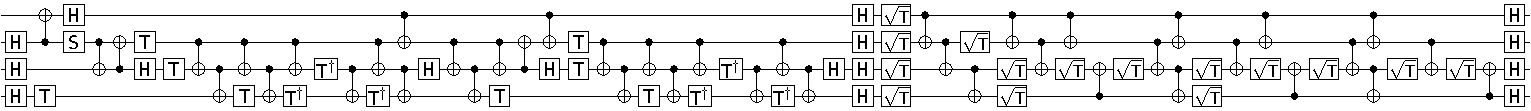
\includegraphics[width=\textwidth]{qnr17_nn.pdf}

\begin{columns}[t]
\separatorcolumn

\begin{column}{\colwidth}

  \begin{block}{An unsolved problem since Gauss}
  \begin{minipage}[c]{0.3\colwidth}
    \includegraphics[width=.25\colwidth]{gauss.jpeg}
  \end{minipage}
  \begin{minipage}[l]{0.7\colwidth}
    \heading{Quadratic nonresidue problem (\csword{QNR}):}
    \bigskip

    Given a prime $p\equiv 1\bmod 8$, find a $y$ such that $x^2\equiv y \bmod p$ has no solution.  

    \bigskip
  {\bf Question:} Is \QNR in \xP?
    \bigskip
  \end{minipage}

Gauss proved the first nontrivial upper bound for the least quadratic nonresidue showing that $y<2\sqrt{p}+1$.
The current best analytic tools prove that $y < C\cdot p^\alpha$ for a non-zero $\alpha$.
  \end{block}

  \begin{exampleblock}{\QNR is in \EQPC}

\begin{algorithm}
  \caption{
    % {\bf Exact quantum polynomial time algorithm for finding a quadratic nonresidues for $p\equiv 1 \bmod 8$.}
    Given $p\equiv 1 \bmod 8$, 
  choose least $n$ where $p<2^n=N$. 
    Let $\theta=\mbox{arccos}\left(1-\frac{2^n}{p-1}\right)$, and
    $f(x)=\left[\jacobi{x}{p}=-1\text{ and } 0\le x<p\right]$.
    % Let $n, N, \theta, x_0 \text{ and } f(x)$ be defined as in section~\ref{qc_alg}.
    % Let $f$ be as defined in equation~\eqref{indicator} and $\theta=\mbox{arccos}\left(1-\frac{N}{p-1}\right)$.
}
  \label{quantum_qnr}
  \begin{noindqlist}
  \item $[O(n)]$ Apply $H^{\otimes n}$ to \( \ket{0}^{\otimes n} \) (Hadamard transform).
    \[ \frac{1}{\sqrt{N}}\sum_{x=0}^{N-1} \ket{x} \]
  \item $[O(n\log^2 n)]$ Compute Jacobi symbol indicator.
\[\frac{1}{\sqrt{N}} \sum_{x=0}^{N-1} \ket{x}\ket{\left[\jacobi{x}{p}=-1\right]}\]
\item $[O(n)]$ Compute the indicator for $[x<p]$.
\[\frac{1}{\sqrt{N}} \sum_{x=0}^{N-1} \ket{x}\ket{\left[\jacobi{x}{p}=-1\right]}\ket{[x<p]}\]
  \item $[O(1)]$ Rotate odd QNRs less than $p$ by $-2\theta$.
  % \item $[O(1)]$ Rotate odd QNRs less than $p$ by $-2\theta$, conditioned on $[x<p],\left[\jacobi{x}{p}=-1\right],$ and $x_0$.
  \[\frac{1}{\sqrt{N}} \sum_{x=0}^{N-1} e^{-i2\theta f(x)x_0}\ket{x}\ket{\left[\jacobi{x}{p}=-1\right]}\ket{[x<p]}\]
\item $[O(1)]$ Rotate all QNRs less than $p$ by $\theta$.
% \item $[O(1)]$ Rotate all QNRs less than $p$ by $\theta$, conditioned on $[x<p]$ and $\left[\jacobi{x}{p}=-1\right]$.
  \[\frac{1}{\sqrt{N}} \sum_{x=0}^{N-1} e^{i\theta f(x)(1-2x_0)}\ket{x}\ket{\left[\jacobi{x}{p}=-1\right]}\ket{[x<p]}\]
\item $[O(n\log^2 n)]$ Uncompute indicator functions.
  \[\frac{1}{\sqrt{N}} \sum_{x=0}^{N-1} e^{i\theta f(x)(1-2x_0)}\ket{x}\]
\item $[O(n)]$ Use a Grover step to invert about the mean $\alpha=\frac{1}{2\sqrt{N}}$.
    \[ \frac{1}{\sqrt N}\sum_{x=0}^{N-1} \left(1-e^{i\theta f(x) (1-2x_0)}\right)\ket{x} \]
  \item $[O(n)]$ Observe a quadratic nonresidue modulo $p$.
  \end{noindqlist}
\end{algorithm}

  \end{exampleblock}
\end{column}

\separatorcolumn

\begin{column}{\colwidth}

  \begin{block}{Phase inversion in the \QNR algorithm}
      \centering
    \begin{figure*}
      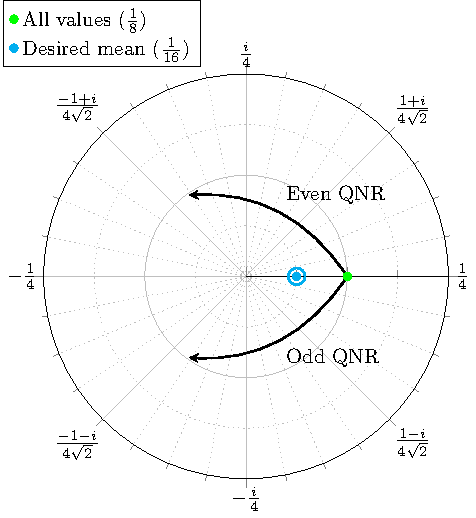
\includegraphics[width=.3\colwidth]{41polar_1.pdf}
    \hfill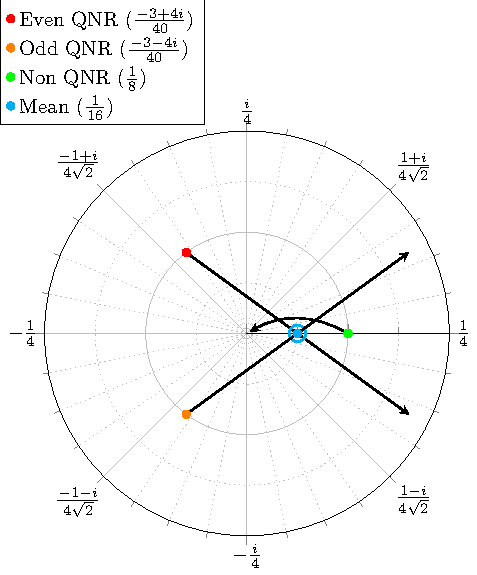
\includegraphics[width=.3\colwidth]{41polar_2.pdf}
    \hfill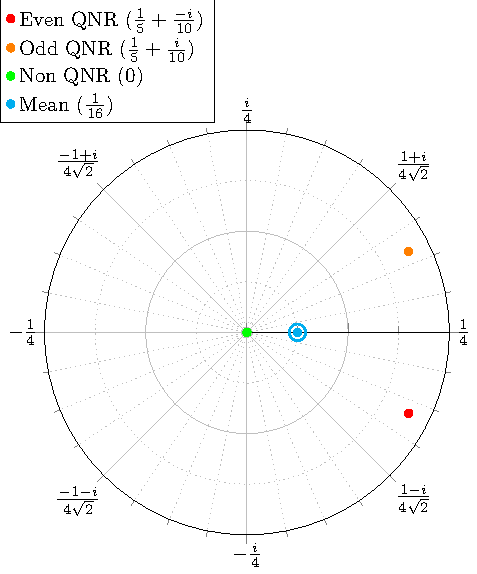
\includegraphics[width=.3\colwidth]{41polar_3.pdf}
      \caption{Amplitude values for Quadratic Nonresidues for $p=41$}
    \end{figure*}

  \end{block}

  \begin{block}{Creating a NISQ test from the \QNR algorithm}
    Using a single Jacobi symbol calculation, a quantum computer can find a \QNR 100\% of the time, 
    whereas a classical computer can only succeed 75\% of the time.

    Even if we want to argue for a different classical bound, without a mathematical breakthrough,
    the provable success rate of any algorithm in \xP will always be less than 100\%.

    A NISQ test based on the \QNR algorithm evaluates two properties:
    % Furthermore, note that the \QNR algorithm produces an equal superposition of \QNR states.
    % This allows two separate NISQ tests:
    \begin{itemize}
      \item The rate of success.
      \item The uniformity of the observations.
    \end{itemize}
  \end{block}



  \begin{block}{Designing a \QNR test circuit for $p=17$}

% \begin{figure}[h]
% \centering
  % 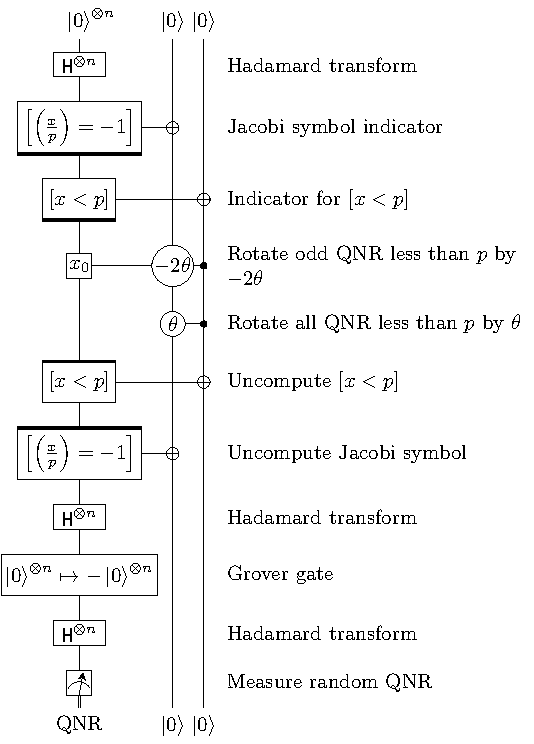
\includegraphics[scale=3]{gen_alg2.pdf}
  % \caption{Wire diagram for algorithm~\ref{quantum_qnr} for sampling quadratic nonresidues}
% \label{fig:gen_alg}
% \end{figure}
  \end{block}

\end{column}

\separatorcolumn

\begin{column}{\colwidth}

  \begin{exampleblock}{A highlighted block containing some math}

    A different kind of highlighted block.

    $$
    \int_{-\infty}^{\infty} e^{-x^2}\,dx = \sqrt{\pi}
    $$

    Interdum et malesuada fames $\{1, 4, 9, \ldots\}$ ac ante ipsum primis in
    faucibus. Cras eleifend dolor eu nulla suscipit suscipit. Sed lobortis non
    felis id vulputate.

    \heading{A heading inside a block}

    Praesent consectetur mi $x^2 + y^2$ metus, nec vestibulum justo viverra
    nec. Proin eget nulla pretium, egestas magna aliquam, mollis neque. Vivamus
    dictum $\mathbf{u}^\intercal\mathbf{v}$ sagittis odio, vel porta erat
    congue sed. Maecenas ut dolor quis arcu auctor porttitor.

    \heading{Another heading inside a block}

    Sed augue erat, scelerisque a purus ultricies, placerat porttitor neque.
    Donec $P(y \mid x)$ fermentum consectetur $\nabla_x P(y \mid x)$ sapien
    sagittis egestas. Duis eget leo euismod nunc viverra imperdiet nec id
    justo.

  \end{exampleblock}

  \begin{block}{References}

    \nocite{*}
    \footnotesize{\bibliographystyle{plain}\bibliography{poster}}

  \end{block}

\end{column}
\separatorcolumn

\begin{column}{\colwidth}
  \begin{block}{Test results for $p=17$ \hspace{1ex}  (Jun-Aug 2021)}
    \heading{Success rates of 1000 shot runs}
    % \raisebox{1mm}[0pt][0pt]{%
      % \makebox[\colwidth][c]{%
    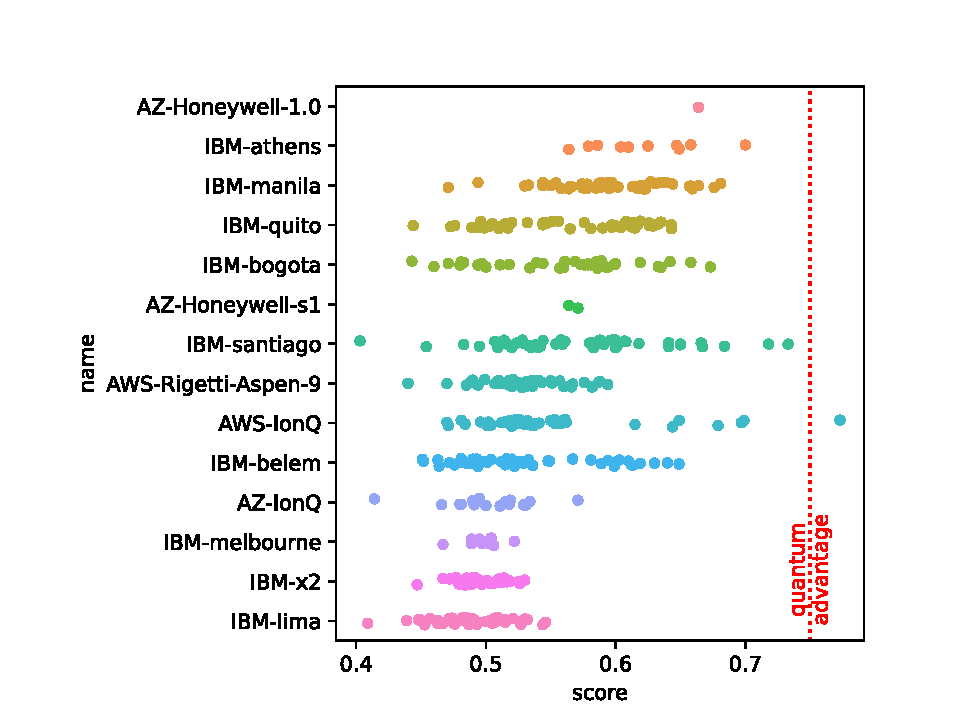
\includegraphics[width=\colwidth]{nisq_stripplot.pdf}
    % }}
    \heading{$p$-values of 1000 shot runs}
    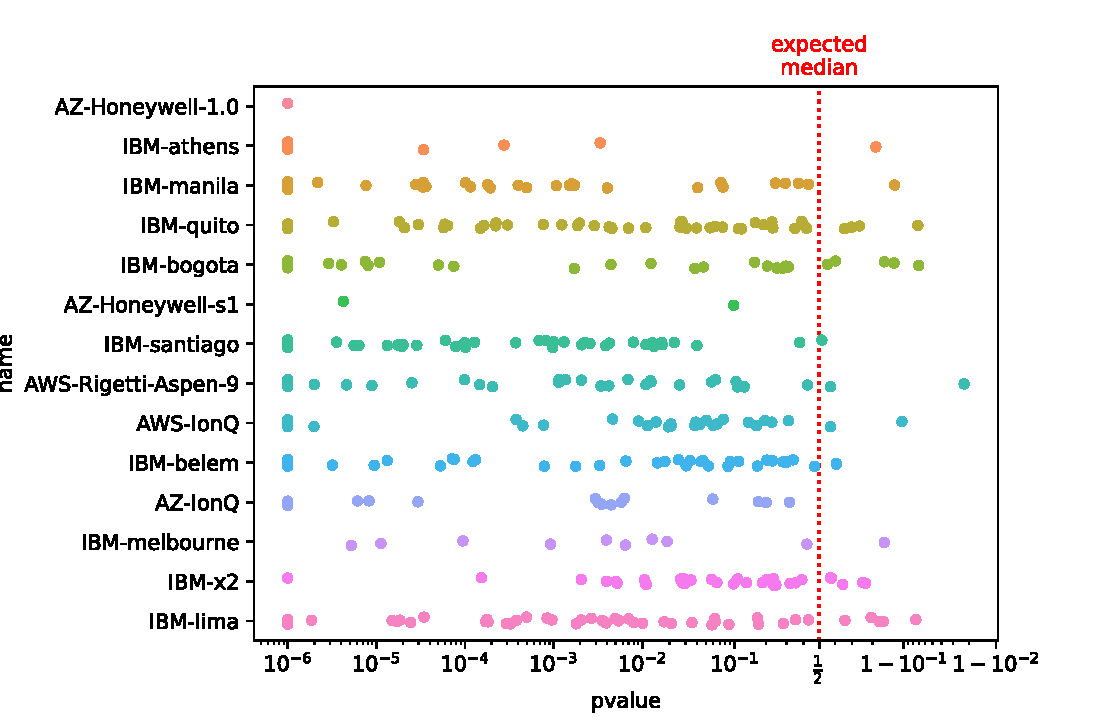
\includegraphics[width=\colwidth]{nisq_pvalue_logit.pdf}
    \heading{Success rate vs. $p$-value}
    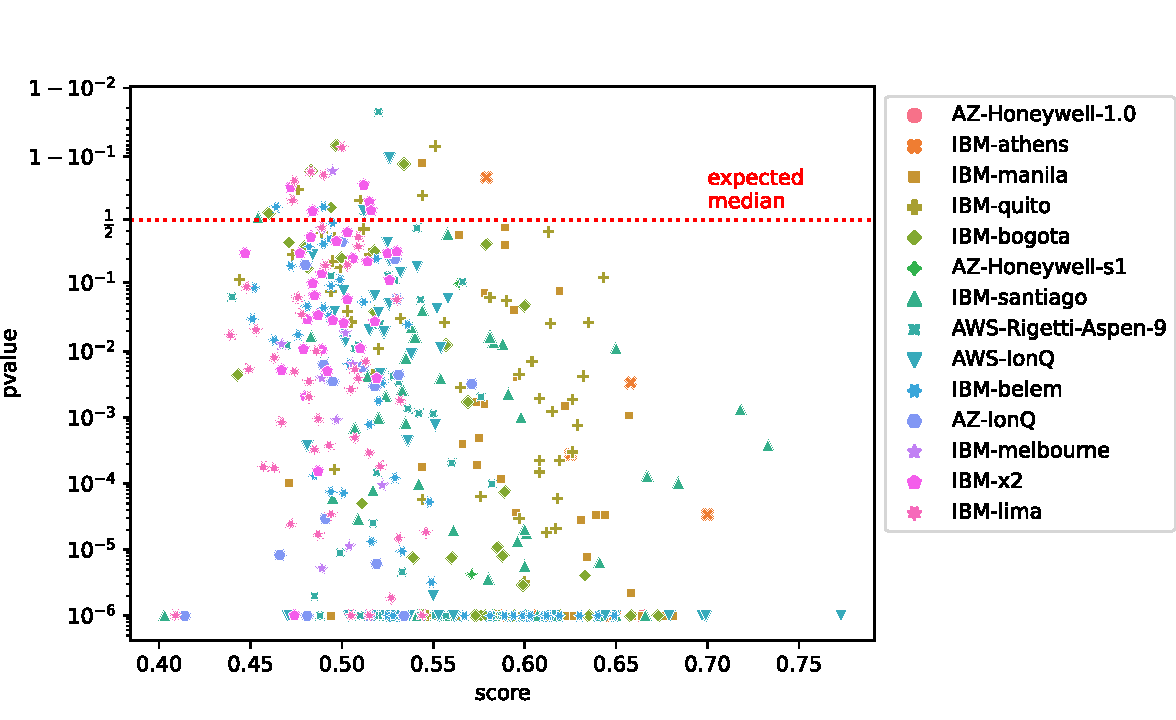
\includegraphics[width=\colwidth]{nisq_scatter.pdf}

  \end{block}


  \begin{block}{References}

    \nocite{*}
    \footnotesize{\bibliographystyle{plain}\bibliography{poster}}

  \end{block}

\end{column}

\separatorcolumn

\begin{column}{\circwidth}
  \begin{block}{Circuit}
    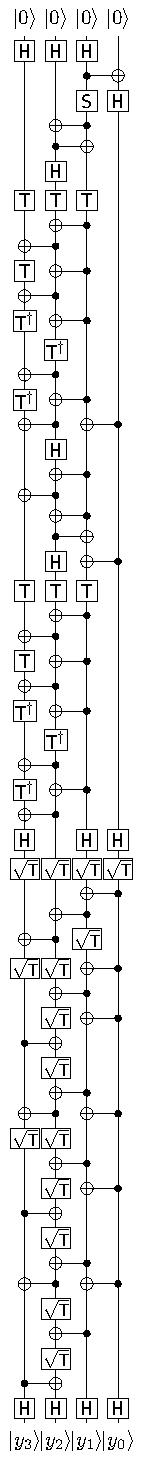
\includegraphics[width=\circwidth]{V4_qnr17_nn.pdf}
  \end{block}

\end{column}

\separatorcolumn
\end{columns}
\end{frame}

\end{document}
